% Provenance (never printed): see sources/outline_sources.md (Year 1: the general
% circulation of the atmosphere, Hadley, Ferrel and polar cells, the ITCZ, Walker cells,
% jet streams, the geostrophic wind, depressions and anticyclones). Exercise and problem
% values in the Book 3 scratch calculator calc/ch28.py; figures from
% figdata/bachelor-1/angular_momentum_wind.py, weather_map.py (an invented map) and
% general_circulation.py (NCEP-NCAR Reanalysis 1, long-term means 1991-2020, datasets
% bachelor-1-ncep-{uwnd-p,vwnd-p,uwnd-sfc,slp,prate-monthly}).
% Physics owns the Coriolis force and the hydrostatic relation (recalled). Book 1 (g8) gave
% the global winds, the convection cell, depressions and anticyclones, isobars and the
% rotation of the wind around them, in words: re-founded here with forces and data.
% ENSO and the monsoons are the Year 2 volume's; the thermal wind the Year 3 volume's.
\chapter{पृथ्वी के वायुमंडल का सामान्य परिसंचरण}\label{ch:b1:atmospheric-circulation}

नौकायन जहाज़ जो यूरोप और अफ़्रीका से अमेरिका की ओर पार करते थे, उष्णकटिबंधों की स्थायी पूर्वी हवाओं, व्यापारिक पवनों, पर निर्भर थे। भूमध्य रेखा के निकट, उसके लगभग पाँच अंश के भीतर, वही पवनें थम जाती थीं, शांति और लगातार बौछारों की उस पट्टी में जिसे नाविक डॉलड्रम्स कहते थे। दोनों के बहुत ऊपर, लगभग नौ किलोमीटर ऊँचाई पर, जेट धाराएँ कही जाने वाली वायु की संकरी नदियाँ \qty{440}{km/h} से अधिक वेग से बह सकती हैं। यह अध्याय तीनों की व्याख्या करता है: घूमते ग्रह पर गतिमान वायु समदाब-रेखाओं के आर-पार नहीं, उनके साथ-साथ क्यों बहती है, उष्णकटिबंधों का आधिक्य भूमध्य रेखा के दोनों ओर एक विशाल पलटने वाला परिसंचरण-कोष्ठ कैसे चलाता है, और भूमध्य रेखा से ऊपर निकलने वाली वायु पश्चिमी जेट में कैसे बदल जाती है।
% ledger: nos:trade-winds, nos:doldrums, noaajs:jet

\begin{omfigure}
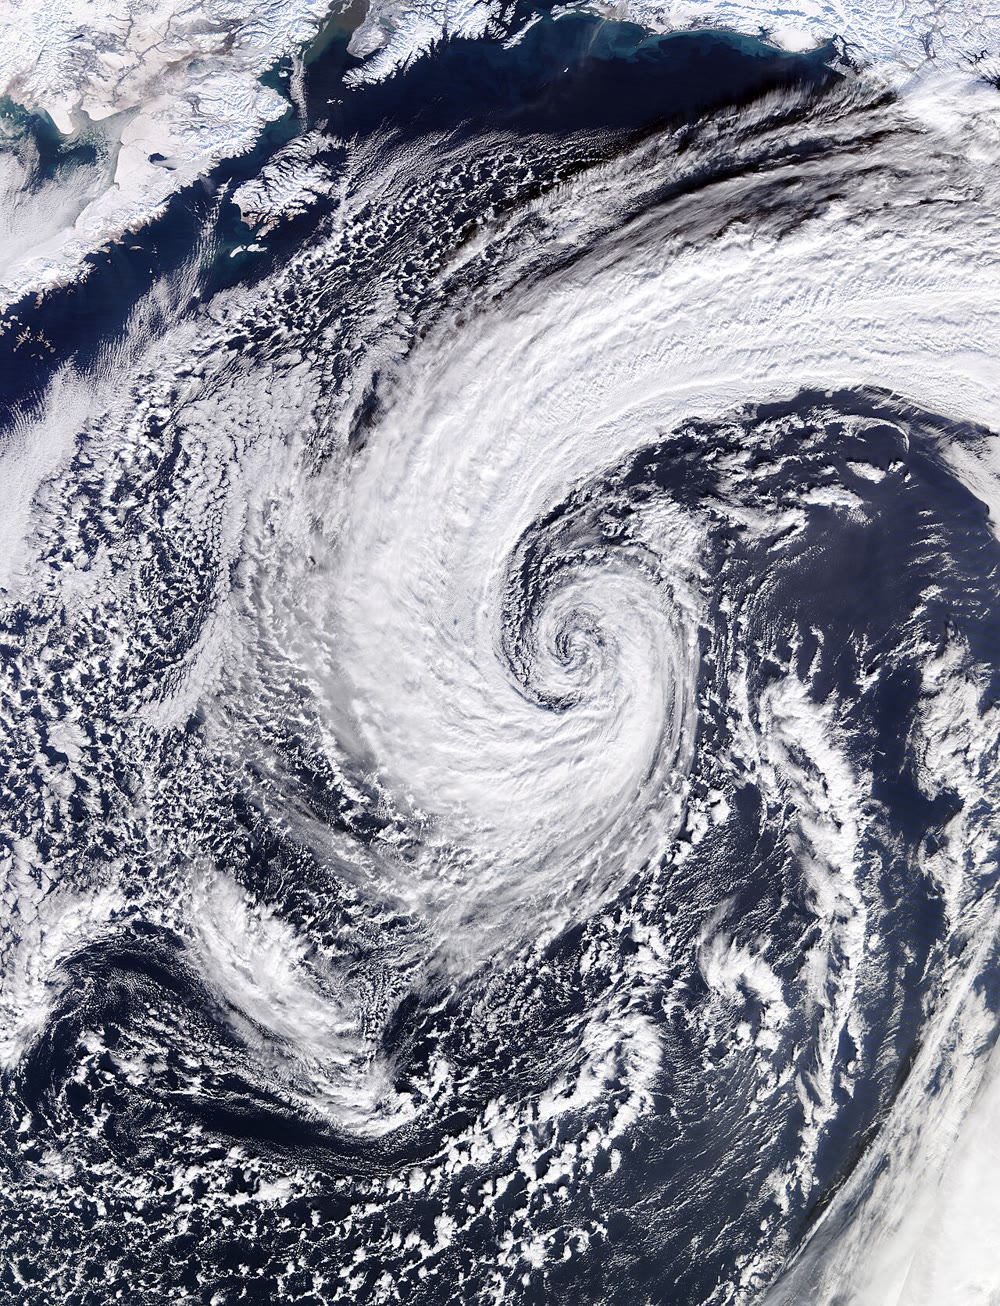
\includegraphics[width=0.5\linewidth]{images/book3/b1-alaska-low.jpg}

{\small 28 जनवरी 2018 को अलास्का की खाड़ी के ऊपर एक बाह्योष्ण \omterm{def:b1:atmospheric-circulation:cyclone}{चक्रवात}, कक्षा से MODIS उपकरण द्वारा देखा गया; अलास्का का हिम-आच्छादित तट ऊपर बाईं ओर है, और उत्तर लगभग ऊपर है। मेघ-पट्टियाँ केंद्र की ओर वामावर्त कुंडली बनाती हैं, जैसे उत्तरी गोलार्ध के अवदाब की वायु करती है। (फ़ोटो: NASA, MODIS/LANCE, सार्वजनिक डोमेन, विकिमीडिया कॉमन्स के माध्यम से।)}
\label{fig:b1:atmospheric-circulation:alaska}
\end{omfigure}
% ledger: commons:alaska-low, nws:cyclone

\begin{recall}
भौतिकी खंड स्थैतिक संबंध और कोरिऑलिस बल देते हैं: एक ऐसे चौखटे में जो कोणीय वेग $\vec\Omega$ से घूमता है, द्रव्यमान $m$ का पिंड जो चौखटे के सापेक्ष वेग $\vec v$ से चलता है, काल्पनिक बल
$-2m\,\vec\Omega\times\vec v$ अनुभव करता है, जो उसकी गति के समकोण पर है। पृथ्वी के लिए, $\Omega = 2\pi/T_\star$ नक्षत्र-दिवस $T_\star = \qty{23.9345}{h}$ के साथ, यानी
$\Omega = \qty{7.292e-5}{rad.s^{-1}}$। पुस्तक~1 ने वैश्विक पवनों का वर्णन किया (\omterm{def:b1:atmospheric-circulation:winds}{व्यापारिक पवनें}, \omterm{def:b1:atmospheric-circulation:winds}{पछुआ पवनें}, ध्रुवीय पूर्वी पवनें), संवहन-कोष्ठ, अवदाब और \omterm{def:b1:atmospheric-circulation:cyclone}{प्रतिचक्रवात}, मौसम-मानचित्र की समदाब-रेखाएँ, और केंद्रों के चारों ओर पवन का मुड़ना। \Cref{ch:b1:fluid-envelopes-structure} ने \omterm{def:b1:fluid-envelopes-structure:standard-atmosphere}{मानक वायुमंडल} और \omterm{def:b1:fluid-envelopes-structure:lapse-rate}{शुष्क रुद्धोष्म तापह्रास दर} दी, और \cref{ch:b1:radiation-heat-transport} ने वह ध्रुवोन्मुखी ऊष्मा परिवहन दिया जो परिसंचरण ले जाता है।
% ledger: earth:Trot, nws:coriolis
\end{recall}

\section{गतिमान वायु पर बल}\label{sec:b1:atmospheric-circulation:forces}

\omterm{def:b1:fluid-envelopes-structure:parcel}{वायु-पिंड} को उसके चारों ओर की वायु का दबाव धकेलता है, गुरुत्व खींचता है, सतह के निकट घर्षण उसे धीमा करता है, और घूमती पृथ्वी से देखने पर कोरिऑलिस बल उसे विक्षेपित करता है। गुरुत्व और ऊर्ध्वाधर दाब-बल लगभग ठीक एक-दूसरे को संतुलित करते हैं: यही स्थैतिक संबंध है। मौसम उन बलों से बनता है जो क्षैतिज में बचे रहते हैं।

\begin{definition}[दाब-प्रवणता बल]\label{def:b1:atmospheric-circulation:pgf}
\emph{दाब-प्रवणता बल}\index{दाब-प्रवणता बल} वह शुद्ध बल है जो तरल-पिंड पर उसके चारों ओर के तरल के दबाव से लगता है। प्रति इकाई द्रव्यमान यह $-(1/\rho)\nabla p$ है, जहाँ $\rho$ घनत्व है और $\nabla p$ दाब-प्रवणता: यह उच्च दाब से निम्न दाब की ओर, समदाब-रेखाओं के आर-पार इशारा करता है।
\end{definition}
% ledger: nws:geostrophic

\begin{proposition}[दाब-प्रवणता बल]\label{prop:b1:atmospheric-circulation:pgf}
$\mathrm dV$ आयतन और $\rho$ घनत्व के \omterm{def:b1:fluid-envelopes-structure:parcel}{वायु-पिंड} पर आसपास के तरल का दबाव बल $-\nabla p\,\mathrm dV$ लगाता है, यानी त्वरण $-(1/\rho)\nabla p$।
\end{proposition}

\begin{proof}
एक छोटा घन लें जिसके किनारे अक्षों के अनुदिश $\mathrm dx$, $\mathrm dy$, $\mathrm dz$ हैं।
$x$ पर के फलक पर दबाव $+x$ दिशा में बल $p(x)\,\mathrm dy\,\mathrm dz$ से धकेलता है; $x + \mathrm dx$ पर के फलक पर, $-x$
दिशा में $p(x + \mathrm dx)\,\mathrm dy\,\mathrm dz$ से। $x$ के अनुदिश शुद्ध बल
$[p(x) - p(x + \mathrm dx)]\,\mathrm dy\,\mathrm dz = -(\partial p/\partial
x)\,\mathrm dV$ है, और इसी प्रकार $y$ और $z$ के अनुदिश। कुल $-\nabla p\,
\mathrm dV$ है; द्रव्यमान $\rho\,\mathrm dV$ से भाग देने पर त्वरण मिलता है।
\end{proof}

एकसमान दबाव कोई शुद्ध बल नहीं लगाता: केवल उसके अंतर धकेलते हैं। मौसम-मानचित्र पर क्षैतिज प्रवणता समदाब-रेखाओं से पढ़ी जाती है: उसका परिमाण दो समदाब-रेखाओं के बीच दाब-अंतर को उनकी दूरी से भाग देने पर मिलता है। समुद्र-तल पर, \qty{4}{hPa} दूर और \qty{400}{km} दूर समदाब-रेखाओं के लिए, जहाँ $\rho \approx \qty{1.225}{kg.m^{-3}}$, त्वरण $400/(1.225 \times \num{4e5}) = \qty{8.2e-4}{m.s^{-2}}$ है, $g$ के दस-हज़ारवें भाग से कम, फिर भी साढ़े तीन घंटों में वायु को विराम से \qty{10}{m/s} तक लाने के लिए पर्याप्त।
% ledger: ussa76:sea-level

वायु कोरिऑलिस बल अनुभव करती है क्योंकि उसे घूमती पृथ्वी से देखा जाता है। उसका क्षैतिज भाग \omterm{def:b1:spherical-astronomy:geographic}{अक्षांश} पर एक ही संख्या के माध्यम से निर्भर करता है।

\begin{definition}[कोरिऑलिस प्राचल]\label{def:b1:atmospheric-circulation:coriolis-parameter}
\emph{कोरिऑलिस प्राचल}\index{कोरिऑलिस प्राचल} \omterm{def:b1:spherical-astronomy:geographic}{अक्षांश} $\varphi$ पर
$f = 2\Omega\sin\varphi$ है, जहाँ $\Omega$ पृथ्वी का कोणीय वेग है। वह उत्तरी गोलार्ध में धनात्मक, दक्षिणी में ऋणात्मक, भूमध्य रेखा पर शून्य, और ध्रुवों पर सबसे बड़ा है,
$2\Omega = \qty{1.458e-4}{s^{-1}}$।
\end{definition}
% ledger: earth:Trot

\begin{proposition}[क्षैतिज कोरिऑलिस त्वरण]\label{prop:b1:atmospheric-circulation:coriolis}
एक क्षैतिज पवन $\vec v$ के लिए, \omterm{def:b1:spherical-astronomy:geographic}{अक्षांश} $\varphi$ पर, कोरिऑलिस त्वरण का क्षैतिज भाग $-f\,\vec k\times\vec v$ है, जहाँ $\vec k$ ऊर्ध्वाधर ऊपर की दिशा है: उसका परिमाण $|f|\,|\vec v|$ है और वह पवन के समकोण पर इंगित करता है, उत्तरी गोलार्ध में उसके दाईं ओर और दक्षिणी में बाईं ओर।
\end{proposition}

\begin{proof}
स्थानीय अक्ष लें: $x$ पूर्व, $y$ उत्तर, $z$ ऊपर। पृथ्वी का घूर्णन-सदिश मध्याह्न-तल में है, उत्तरी क्षितिज के ऊपर कोण $\varphi$ पर: $\vec\Omega =
\Omega(0, \cos\varphi, \sin\varphi)$। $\vec v = (u, v, 0)$ के लिए,
\[
  \vec\Omega\times\vec v = \Omega\,(-v\sin\varphi,\ u\sin\varphi,\ -u\cos\varphi),
  \qquad -2\vec\Omega\times\vec v = (f v,\ -f u,\ 2\Omega u\cos\varphi).
\]
$\vec k\times\vec v = (-v, u, 0)$ होने से, क्षैतिज भाग $(fv, -fu)$
$-f\,\vec k\times\vec v$ है। सदिश $\vec k\times\vec v$ वह $\vec v$ है जो ऊपर से देखने पर वामावर्त \ang{90} घुमाया गया हो; उसका विलोम $\vec v$ है जो दक्षिणावर्त घुमाया गया हो,
दाईं ओर, जब $f > 0$, और बाईं ओर, जब $f < 0$।
\end{proof}
% ledger: earth:Trot

ऊर्ध्वाधर भाग, $2\Omega u\cos\varphi$, \qty{10}{m/s} की पवन के लिए अधिक से अधिक \qty{1.5e-3}{m.s^{-2}} है, $g$ का लगभग \num{1.5e-4}: स्थैतिक संतुलन उसे सोख लेता है। क्षैतिज भाग, छोटा होते हुए भी, घर्षण-परत के ऊपर मुक्त वायुमंडल में कोई प्रतिद्वंद्वी नहीं रखता, और घंटों में हर पवन को आकार देता है।

सतह के निकट वायु सतह से भी रगड़ खाती है। सबसे निचले किलोमीटर में, मौसम-विज्ञानियों की घर्षण-परत में, घर्षण पवन की गति और दिशा दोनों बदलता है; विक्षुब्ध भँवर सतह का खिंचाव ऊपर की ओर ले जाते हैं, और बल मोटे तौर पर पवन के विरुद्ध कार्य करता है और उसके साथ बढ़ता है। ऊपर, मुक्त वायुमंडल में, घर्षण छोटा है।
% ledger: nws:friction-layer

\section{भू-विक्षेपी पवन}\label{sec:b1:atmospheric-circulation:geostrophic}

\begin{definition}[भू-विक्षेपी संतुलन, भू-विक्षेपी पवन]\label{def:b1:atmospheric-circulation:geostrophic}
एक क्षैतिज प्रवाह \emph{भू-विक्षेपी संतुलन}\index{भू-विक्षेपी संतुलन} में है जब उसका \omterm{def:b1:atmospheric-circulation:pgf}{दाब-प्रवणता बल} और उसका कोरिऑलिस बल एक-दूसरे को निरस्त करते हैं। \emph{भू-विक्षेपी पवन}\index{भू-विक्षेपी पवन} $\vec v_g$ वह पवन है जो किसी दिए गए दाब-क्षेत्र के लिए यह संतुलन प्राप्त करती है:
$-(1/\rho)\nabla p - f\,\vec k\times\vec v_g = \vec 0$।
\end{definition}
% ledger: nws:geostrophic

\begin{theorem}[भू-विक्षेपी पवन]\label{thm:b1:atmospheric-circulation:geostrophic}
भूमध्य रेखा से दूर,
\[
  \vec v_g = \frac{1}{\rho f}\,\vec k\times\nabla p, \qquad
  |\vec v_g| = \frac{|\nabla p|}{\rho\,|f|} .
\]
\omterm{def:b1:atmospheric-circulation:geostrophic}{भू-विक्षेपी पवन} समदाब-रेखाओं के साथ बहती है, जहाँ वे पास हों वहाँ तेज़। उत्तरी गोलार्ध में वह निम्न दाब को अपनी बाईं ओर रखती है; दक्षिणी गोलार्ध में, दाईं ओर।
\end{theorem}

\begin{proof}
क्षैतिज सदिश $\vec w$ के लिए, $\vec k\times(\vec k\times\vec w) = -\vec w$।
$\vec k\times$ को संतुलन $f\,\vec k\times\vec v_g = -(1/\rho)\nabla p$ पर लगाने पर
$-f\vec v_g = -(1/\rho)\,\vec k\times\nabla p$ मिलता है, अतः सूत्र, जो वहाँ मान्य है जहाँ
$f \neq 0$ है। चूँकि $\vec k\times\nabla p$ $\nabla p$ पर लंबवत है, पवन प्रवणता के लंबवत है, यानी समदाब-रेखाओं के अनुदिश; उसका परिमाण $|\nabla
p|/(\rho|f|)$ है। सदिश $\vec k\times\nabla p$ वह प्रवणता है जो \ang{90} वामावर्त घुमाई गई हो। उसकी दिशा में मुँह करके, प्रवणता, जो उच्च दाब की ओर इंगित करती है, दाईं ओर पड़ती है, इसलिए निम्न दाब बाईं ओर है; $f > 0$ के लिए पवन की दिशा $\vec k\times\nabla p$ की है, $f < 0$ के लिए विपरीत।
\end{proof}

\begin{example}[समदाब-रेखाओं से पढ़ी गई पवन]\label{ex:b1:atmospheric-circulation:geostrophic}
\ang{50} उ पर, $f = 2 \times \num{7.292e-5} \times \sin\ang{50} = \qty{1.117e-4}{s^{-1}}$।
\qty{4}{hPa} दूर और \qty{400}{km} दूर समदाब-रेखाएँ $|\nabla p| = 400/\num{4e5} =
\qty{1.0e-3}{Pa.m^{-1}}$ देती हैं, और $\rho = \qty{1.225}{kg.m^{-3}}$ के साथ, एक \omterm{def:b1:atmospheric-circulation:geostrophic}{भू-विक्षेपी
पवन} $\num{1.0e-3}/(1.225 \times \num{1.117e-4}) = \qty{7.3}{m/s}$ है। वही अंतर \ang{20} उ पर, जहाँ $f$ आधे से कम है, \qty{16.4}{m/s} देता।
\end{example}
% ledger: earth:Trot, ussa76:sea-level

संतुलन तात्कालिक नहीं है। दाब-प्रवणता से चलाई गई वायु कोरिऑलिस बल के तले दर $f$ से मुड़ती है, लगभग हर $2\pi/f$ पर एक बार, \ang{50} पर लगभग सोलह घंटे; कुछ घंटों से अधिक चलने वाले और कुछ सौ किलोमीटर से बड़े प्रतिरूप भू-विक्षेपी के निकट हैं। भूमध्य रेखा के निकट $f$ शून्य की ओर जाता है, सूत्र विफल होता है, और गहरे उष्णकटिबंध की पवनें भू-विक्षेपी नहीं हैं।

\begin{omfigure}
\begin{tikzpicture}[>={Stealth[length=2.2mm]}, font=\scriptsize]
  % left panel: geostrophic balance
  \begin{scope}
    \draw[isobar] (-2.4,1.2) -- (2.4,1.2) node[right] {\qty{996}{hPa}};
    \draw[isobar] (-2.4,0) -- (2.4,0) node[right] {\qty{1000}{hPa}};
    \draw[isobar] (-2.4,-1.2) -- (2.4,-1.2) node[right] {\qty{1004}{hPa}};
    \node[pressure low] at (0,2.0) {L};
    \node[pressure high] at (0,-2.0) {H};
    \fill (0,0) circle (1.6pt);
    \draw[->, very thick, omThm] (0,0) -- (0,1.0);
    \node[omThm, anchor=east] at (-0.08,0.6) {दाब-प्रवणता};
    \draw[->, very thick, omDef] (0,0) -- (0,-1.0);
    \node[omDef, anchor=east] at (-0.08,-0.6) {कोरिऑलिस};
    \draw[->, line width=1.6pt, black] (0,0) -- (1.9,0) node[above, pos=0.75] {पवन $\vec v_g$};
    \node[anchor=north] at (0,-2.4) {घर्षण के बिना: भू-विक्षेपी संतुलन};
  \end{scope}
  % right panel: with friction (alpha = 25 deg, V = Vg cos alpha)
  \begin{scope}[xshift=7.4cm]
    \draw[isobar] (-2.4,1.2) -- (2.4,1.2) node[right] {\qty{996}{hPa}};
    \draw[isobar] (-2.4,0) -- (2.4,0) node[right] {\qty{1000}{hPa}};
    \draw[isobar] (-2.4,-1.2) -- (2.4,-1.2) node[right] {\qty{1004}{hPa}};
    \node[pressure low] at (0,2.0) {L};
    \node[pressure high] at (0,-2.0) {H};
    \fill (0,0) circle (1.6pt);
    \draw[->, very thick, omThm] (0,0) -- (0,1.0);
    \node[omThm, anchor=east] at (-0.08,0.6) {दाब-प्रवणता};
    \draw[->, very thick, omDef] (0,0) -- ({1.0*cos(25)*sin(25)},{-1.0*cos(25)*cos(25)});
    \node[omDef, anchor=west] at (0.42,-0.62) {कोरिऑलिस};
    \draw[->, very thick, omMeth] (0,0) -- ({-1.0*sin(25)*cos(25)},{-1.0*sin(25)*sin(25)})
      node[below left, inner sep=1pt] {घर्षण};
    \draw[->, line width=1.6pt, black] (0,0) -- ({1.9*cos(25)*cos(25)},{1.9*cos(25)*sin(25)})
      node[above, inner sep=2pt] {पवन $\vec v$};
    \draw[black!50, dashed] (0,0) -- (1.9,0);
    \draw[black!60] (1.0,0) arc[start angle=0, end angle=25, radius=1.0];
    \node[black!70] at (1.22,0.22) {$\alpha$};
    \node[anchor=north] at (0,-2.4) {घर्षण के साथ: धीमी, समदाब-रेखाओं के आर-पार};
  \end{scope}
\end{tikzpicture}

{\small उत्तरी गोलार्ध में \omterm{def:b1:fluid-envelopes-structure:parcel}{वायु-पिंड} पर बल, निम्न दाब उत्तर में। बाईं ओर: मुक्त वायुमंडल में \omterm{def:b1:atmospheric-circulation:pgf}{दाब-प्रवणता बल} (लाल) और कोरिऑलिस बल (नीला) एक-दूसरे को निरस्त करते हैं, और पवन समदाब-रेखाओं के साथ बहती है, निम्न उसकी बाईं ओर। दाईं ओर: सतह के निकट घर्षण (हरा) पवन के विरुद्ध कार्य करता है; तीनों बल तभी संतुलित होते हैं जब पवन धीमी हो और कोण $\alpha$ से निम्न की ओर मुड़ी हो ($\alpha = \ang{25}$ के लिए खींचा गया, और \cref{prop:b1:atmospheric-circulation:friction} के खिंचाव के लिए)।}
\label{fig:b1:atmospheric-circulation:balance}
\end{omfigure}

\begin{proposition}[घर्षण पवन को निम्न दाब की ओर मोड़ता है]\label{prop:b1:atmospheric-circulation:friction}
माना एक स्थायी क्षैतिज पवन $\vec v$ पर \omterm{def:b1:atmospheric-circulation:pgf}{दाब-प्रवणता बल} कार्य करता है,
कोरिऑलिस बल, और घर्षण बल $-\vec v/\tau$, जहाँ $\tau > 0$ है, एक ऐसे \omterm{def:b1:spherical-astronomy:geographic}{अक्षांश} पर जहाँ $f > 0$ है। तब पवन समदाब-रेखाओं को निम्न दाब की ओर
कोण $\alpha$ पर पार करती है, जहाँ $\tan\alpha = 1/(f\tau)$ है, और उसकी गति $|\vec v| =
|\vec v_g|\cos\alpha$ है, \omterm{def:b1:atmospheric-circulation:geostrophic}{भू-विक्षेपी पवन} से कम।
\end{proposition}

\begin{proof}
माना $V = |\vec v|$, $\hat v$ पवन के अनुदिश इकाई सदिश और $\hat n$ उसके समकोण पर, उसकी बाईं ओर का इकाई सदिश हो। संतुलन है $-(1/\rho)\nabla p - f\,
\vec k\times\vec v - \vec v/\tau = \vec 0$ है, और $\vec k\times\vec v = V\hat n$।
पवन के अनुदिश $\hat v$ पर: $-(1/\rho)\,\nabla p\cdot\hat v = V/\tau > 0$, इसलिए पवन का एक घटक दाब-प्रवणता के नीचे, निम्न दाब की ओर है। $\hat n$ के अनुदिश:
$-(1/\rho)\,\nabla p\cdot\hat n = fV$। \omterm{def:b1:atmospheric-circulation:pgf}{दाब-प्रवणता बल}, परिमाण $P =
|\nabla p|/\rho = f|\vec v_g|$ है, इसलिए पवन के अनुदिश घटक $V/\tau$ और
$fV$ उसके आर-पार है: वह पवन के साथ कोण $\beta$ बनाता है जिसके लिए $\tan\beta =
1/(f\tau)$, और $P^2 = V^2(f^2 + 1/\tau^2)$। समदाब-रेखाएँ प्रवणता के लंबवत हैं, इसलिए पवन उन्हें $\alpha = \beta$ कोण पर पार करती है, और $V = P/\sqrt{f^2 +
1/\tau^2} = (P/f)\cos\alpha = |\vec v_g|\cos\alpha$।
\end{proof}

अधिक खुरदरी सतह का अर्थ है अधिक खिंचाव, छोटा $\tau$ और बड़ा कोण: पवन समुद्र के ऊपर की तुलना में ज़मीन के ऊपर समदाब-रेखाओं को अधिक तिरछेपन से पार करती है। वास्तविक घर्षण पवन में ठीक रैखिक नहीं है, पर निष्कर्ष, धीमी और निम्न की ओर मुड़ी हुई, सामान्य है।

\begin{remark}[प्रवणता पवन]\label{rem:b1:atmospheric-circulation:gradient}
किसी केंद्र के चारों ओर समदाब-रेखाएँ वक्र होती हैं, और उनका अनुसरण करने वाली वायु वक्रता-केंद्र की ओर त्वरित होती है: $V^2/r$, त्रिज्या $r$ के वृत्त के लिए। उत्तरी गोलार्ध में निम्न के चारों ओर \omterm{def:b1:atmospheric-circulation:pgf}{दाब-प्रवणता बल} को तब कोरिऑलिस बल से अधिक होना चाहिए: $fV + V^2/r = f|\vec v_g|$, और इस पवन को, जिसे प्रवणता-पवन कहते हैं, भू-विक्षेपी से दुर्बल होना चाहिए। \omterm{def:b1:atmospheric-circulation:cyclone}{प्रतिचक्रवात} के चारों ओर कोरिऑलिस बल \omterm{def:b1:atmospheric-circulation:pgf}{दाब-प्रवणता बल} से अधिक होना चाहिए, $fV - V^2/r = f|\vec v_g|$: पवन प्रबल है, पर समीकरण का हल तभी है यदि $|\vec v_g| \leq fr/4$, जो \omterm{def:b1:atmospheric-circulation:cyclone}{प्रतिचक्रवात} के केंद्र के निकट प्रबल दाब-प्रवणताओं को वर्जित करता है (\cref{exo:b1:atmospheric-circulation:10})।
\end{remark}

\section{अवदाब और प्रतिचक्रवात}\label{sec:b1:atmospheric-circulation:cyclones}

\begin{definition}[चक्रवात, प्रतिचक्रवात]\label{def:b1:atmospheric-circulation:cyclone}
\emph{चक्रवात}\index{चक्रवात} निम्न दाब के केंद्र के चारों ओर पवनों का एक बड़े पैमाने का परिसंचरण है, एक अवदाब; \emph{प्रतिचक्रवात}\index{प्रतिचक्रवात} उच्च दाब के केंद्र के चारों ओर का परिसंचरण है। चक्रवात उत्तरी गोलार्ध में वामावर्त और दक्षिणी में दक्षिणावर्त घूमता है; प्रतिचक्रवात उसके उलटी दिशा में।
\end{definition}
% ledger: nws:cyclone

घूर्णन की दिशाएँ \cref{thm:b1:atmospheric-circulation:geostrophic} से आती हैं:
उत्तरी गोलार्ध में, वह पवन जो निम्न को अपनी बाईं ओर रखती है, निम्न के चारों ओर वामावर्त और उच्च के चारों ओर दक्षिणावर्त जाती है। अंतरिक्ष से देखने पर, अवदाब के मेघ घूर्णन का मार्ग दिखाते हैं (अध्याय के आरंभ का चित्र); दक्षिणी गोलार्ध में कुंडलियाँ दर्पण-प्रतिबिंब हैं।
% ledger: nws:cyclone, commons:alaska-low

\begin{history}[बाइस बैलट का नियम, 1857]
1857 में डच मौसम-विज्ञानी C.~H.~D. बाइस बैलट ने प्रेक्षणों में मिलने वाला एक नियम बताया: उत्तरी गोलार्ध में, पवन की ओर पीठ करके खड़े व्यक्ति की बाईं ओर निम्न दाब होता है और दाईं ओर उच्च दाब; दक्षिणी गोलार्ध में, उलटा। उन्होंने यह भी नहीं जाना कि अमेरिकी मौसम-विज्ञानी विलियम फेरेल पहले ही उसे सिद्धांत से निकाल चुके थे, और बाद में फेरेल की प्राथमिकता स्वीकार की।
\omterm{def:b1:atmospheric-circulation:geostrophic}{भू-विक्षेपी पवन} इसी नियम का समीकरणों में रूप है।
\end{history}
% ledger: skybrary:buys-ballot

घर्षण एक महत्वपूर्ण मोड़ जोड़ता है। सतह के निकट पवन समदाब-रेखाओं को निम्न दाब की ओर पार करती है, जैसा (\cref{prop:b1:atmospheric-circulation:friction}): अवदाब के चारों ओर वायु भीतर की ओर कुंडली बनाती है, सतह के निकट अभिसरण करती है, और ऊपर उठना पड़ता है। ऊपर उठती वायु फैलती है और \omterm{def:b1:fluid-envelopes-structure:lapse-rate}{शुष्क रुद्धोष्म तापह्रास दर} पर ठंडी होती है (\cref{ch:b1:fluid-envelopes-structure}), और संतृप्त होते ही उसका जल-वाष्प संघनित होता है: अवदाब मेघ और वर्षा लाते हैं। \omterm{def:b1:atmospheric-circulation:cyclone}{प्रतिचक्रवात} के चारों ओर सतह की वायु बाहर की ओर कुंडली बनाती है; उसकी जगह लेने को ऊपर से वायु नीचे उतरती है, संपीड़न से गरम होती है, और उसके मेघ वाष्पित हो जाते हैं: \omterm{def:b1:atmospheric-circulation:cyclone}{प्रतिचक्रवात} स्थिर, प्रायः साफ़ मौसम लाते हैं।
% ledger: nws:dalr

नीचे का मानचित्र एक काल्पनिक उदाहरण है, प्रेक्षित नहीं बल्कि परिकलित: \qty{28}{hPa} गहरा एक अवदाब और \qty{1013}{hPa} की पृष्ठभूमि पर \qty{20}{hPa} ऊँचा एक \omterm{def:b1:atmospheric-circulation:cyclone}{प्रतिचक्रवात}, जो लगभग \ang{50} उ पर केंद्रित हैं। हर स्टेशन पर पवन-बार्ब वह \omterm{def:b1:atmospheric-circulation:geostrophic}{भू-विक्षेपी पवन} दिखाता है जो मानचित्र से \cref{thm:b1:atmospheric-circulation:geostrophic} के साथ परिकलित हुई।

\begin{omfigure}
\pgfplotstableread{figdata/out/bachelor-1-weather_map-stations.dat}\wmstations
\pgfplotstableread{figdata/out/bachelor-1-weather_map-labels.dat}\wmlabels
\begin{tikzpicture}
\begin{axis}[x=0.0038cm, y=0.0038cm, disabledatascaling, anchor=origin,
  xmin=-1800, xmax=1800, ymin=-1200, ymax=1200, xtick=\empty, ytick=\empty,
  axis background/.style={fill=blue!4}, clip=true]
% figdata/bachelor-1/weather_map.py (invented pressure field); ledger: earth:Trot, ussa76:sea-level
\addplot[isobar, unbounded coords=jump] table[x=x, y=y] {figdata/out/bachelor-1-weather_map-isobars.dat};
\addplot[black!45, dashed, domain=-1800:1800] {0};
\addplot[only marks, mark=none, nodes near coords, point meta=explicit symbolic,
  nodes near coords style={font=\tiny, fill=blue!4, inner sep=0.5pt, anchor=center}]
  table[x=x, y=y, meta=p] {\wmlabels};
\node[pressure low] at (axis cs:-500,150) {L};
\node[pressure high] at (axis cs:1050,-250) {H};
\node[font=\tiny, anchor=south west, black!60] at (axis cs:-1790,5) {\ang{50} उ};
\end{axis}
\pgfplotstablegetrowsof{\wmstations}
\pgfmathtruncatemacro{\wmlast}{\pgfplotsretval-1}
\begin{scope}
\clip (-6.84,-4.56) rectangle (6.84,4.56);
\foreach \i in {0,...,\wmlast}{
  \pgfplotstablegetelem{\i}{x}\of\wmstations \let\wx\pgfplotsretval
  \pgfplotstablegetelem{\i}{y}\of\wmstations \let\wy\pgfplotsretval
  \pgfplotstablegetelem{\i}{speed_kn}\of\wmstations \let\ws\pgfplotsretval
  \pgfplotstablegetelem{\i}{from_deg}\of\wmstations \let\wd\pgfplotsretval
  \pic[transform shape] at ({\wx*0.0038},{\wy*0.0038}) {windbarb={\ws}{\wd}};
}
\end{scope}
\pic[transform shape] at (-6.5,-4.0) {scalebar={1.9}{\qty{500}{km}}};
\pic[scale=0.7, transform shape] at (-6.45,3.2) {northarrow};
\end{tikzpicture}

{\small लगभग \ang{50} उ पर एक काल्पनिक समुद्र-तल दाब मानचित्र (समदाब-रेखाएँ हर \qty{4}{hPa} पर; केंद्रीय दाब \qty{986}{hPa} और \qty{1033}{hPa})। हर बार्ब अपने स्टेशन की \omterm{def:b1:atmospheric-circulation:geostrophic}{भू-विक्षेपी पवन} दिखाता है, दंड उस दिशा की ओर जहाँ से पवन आती है; पूरा पंख \qty{10}{kn}, आधा पंख \qty{5}{kn}, एक झंडा \qty{50}{kn} (\qty{1}{kn} = \qty{0.514}{m/s})। पवनें निम्न के चारों ओर वामावर्त और उच्च के चारों ओर दक्षिणावर्त मुड़ती हैं, और जहाँ दोनों के बीच समदाब-रेखाएँ सघन होती हैं वहाँ सबसे प्रबल हैं, \qty{36}{m/s} तक।}
\label{fig:b1:atmospheric-circulation:weather-map}
\end{omfigure}
% ledger: earth:Trot, ussa76:sea-level (computed in figdata/bachelor-1/weather_map.py)

\section{तीन-कोष्ठ परिसंचरण}\label{sec:b1:atmospheric-circulation:cells}

पूरे गोले पर और कई वर्षों पर औसत लेने पर, उत्तर या दक्षिण की ओर बहने वाली पवनें कमज़ोर हैं, अधिक से अधिक कुछ मीटर प्रति सेकंड, पर वे बहुत वायु ले जाती हैं। उनका प्रतिरूप भूमध्य रेखा और ध्रुवों के बीच बहने वाले द्रव्यमान में सबसे अच्छा दिखता है।

\begin{definition}[माध्य उत्तर-दक्षिण धारा-फलन]\label{def:b1:atmospheric-circulation:streamfunction}
\emph{माध्य उत्तर-दक्षिण धारा-फलन}\index{माध्य उत्तर-दक्षिण धारा-फलन}
$\psi(p, \varphi)$ वह वायु-द्रव्यमान है प्रति सेकंड जो \omterm{def:b1:spherical-astronomy:geographic}{अक्षांश} $\varphi$ को दाब-स्तर $p$ के ऊपर उत्तर की ओर पार करता है, ज़ोनल और काल-माध्य में:
\[
  \psi(p, \varphi) = \frac{2\pi a_\oplus\cos\varphi}{g}\int_0^p [v]\,\mathrm dp' ,
\]
जहाँ $[v]$ समांतर रेखा के चारों ओर माध्य उत्तरी पवन है। यह \unit{kg.s^{-1}} में मापा जाता है।
\end{definition}

हाइड्रोस्टैटिक संबंध से $\mathrm dp' = -\rho g\,\mathrm dz$, इसलिए $2\pi a_\oplus
\cos\varphi\,[v]\,\mathrm dp'/g$ समांतर रेखा के एक वलय के आर-पार द्रव्य-फ़्लक्स है। वह वायु जो $p$ के ऊपर समांतर रेखा को पार करती है, उसे $p$ के नीचे उलटी दिशा में पार करनी होगी, क्योंकि द्रव्यमान जमा नहीं होता: $\psi$ सतह पर और शीर्ष पर शून्य है, और उसकी समान-मान रेखाएँ माध्य परिसंचरण के पथ हैं। $\psi > 0$ वाला कोष्ठ, जब उत्तरी ध्रुव दाईं ओर रखकर खींचा जाए, दक्षिणावर्त घूमता है: ऊपर उत्तर की ओर, नीचे दक्षिण की ओर।

\begin{omfigure}
\begin{tikzpicture}
\begin{groupplot}[group style={group size=1 by 2, vertical sep=1.3cm},
  width=0.82\linewidth, height=4.6cm, view={0}{90}, xmin=-70, xmax=70, ymin=100,
  ymax=1000, y dir=reverse, ytick={200,400,600,800,1000}, xtick={-60,-40,...,60},
  tick label style={font=\scriptsize}, label style={font=\small},
  ylabel={दाब (\unit{hPa})},
  colormap={omdiv}{rgb255=(33,102,172) rgb255=(146,197,222) rgb255=(247,247,247)
    rgb255=(244,165,130) rgb255=(178,24,43)},
  point meta min=-22, point meta max=22, colorbar,
  colorbar style={width=0.25cm, y dir=normal, ytick={-20,-10,0,10,20}, tick label style={font=\scriptsize},
    ylabel={$\psi$ (\qty{e10}{kg.s^{-1}})}, ylabel style={font=\scriptsize}},
  axis on top, grid=none]
\nextgroupplot[title={दिसंबर--फ़रवरी}, title style={font=\small}]
% figdata/bachelor-1/general_circulation.py; ledger: data:b3-ncep-circ, psl:ncep-r1
\addplot3[surf, shader=interp, mesh/ordering=x varies, mesh/cols=73]
  table[x=lat, y=p, z=psi] {figdata/out/bachelor-1-general_circulation-psi-djf.dat};
\addplot3[black, line width=0.5pt, unbounded coords=jump]
  table[x=lat, y=p, z expr=40] {figdata/out/bachelor-1-general_circulation-psi0-djf.dat};
\nextgroupplot[title={जून--अगस्त}, title style={font=\small}, xlabel={अक्षांश (\unit{\degree})}]
\addplot3[surf, shader=interp, mesh/ordering=x varies, mesh/cols=73]
  table[x=lat, y=p, z=psi] {figdata/out/bachelor-1-general_circulation-psi-jja.dat};
\addplot3[black, line width=0.5pt, unbounded coords=jump]
  table[x=lat, y=p, z expr=40] {figdata/out/bachelor-1-general_circulation-psi0-jja.dat};
\end{groupplot}
\end{tikzpicture}

{\small \omterm{def:b1:atmospheric-circulation:streamfunction}{माध्य उत्तर-दक्षिण धारा-फलन} शीतकालीन उत्तरी (ऊपर) और ग्रीष्मकालीन उत्तरी (नीचे), एनसीईपी-एनसीएआर पुनर्विश्लेषण 1 के ज़ोनल-माध्य उत्तरी पवन से, 1991--2020 के माध्य (डेटा: NOAA PSL)। लाल: इस दृश्य में दक्षिणावर्त कोष्ठ (उनकी दक्षिणी ओर उठते हुए), नीला: वामावर्त; काला: वे शून्य रेखाएँ जो कोष्ठों को अलग करती हैं। शीतकालीन \omterm{def:b1:atmospheric-circulation:cells}{हैडली कोष्ठ} भूमध्य रेखा के आर-पार फैला है और ग्रीष्मकालीन कोष्ठ को बौना कर देता है।}
\label{fig:b1:atmospheric-circulation:psi}
\end{omfigure}
% ledger: data:b3-ncep-circ, psl:ncep-r1 (computed in figdata/bachelor-1/general_circulation.py)

वार्षिक माध्य में पुनर्विश्लेषण भूमध्य रेखा के आर-पार दो प्रबल कोष्ठ दिखाता है, \qty{400}{hPa} पर \ang{15} उ और \ang{15} दक्षिण के निकट \qty{8.7e10}{kg/s} के शिखर के साथ; \qty{500}{hPa} पर उनके ध्रुवीय किनारे \ang{33} उ और \ang{32} दक्षिण पर हैं। उनके ध्रुवों की ओर, दो कमज़ोर कोष्ठ उलटी दिशा में मुड़ते हैं, लगभग \ang{61} उ और \ang{64} दक्षिण तक। ऋतुएँ चित्र को नया रूप देती हैं: दिसंबर से फ़रवरी, उत्तरी शीत, वह कोष्ठ जो भूमध्य रेखा के दक्षिण में उठता है और उत्तरी उपोष्णकटिबंध में नीचे उतरता है, \qty{21.4e10}{kg/s} ले जाता है और \ang{13} दक्षिण से \ang{31} उ तक पहुँचता है; जून से अगस्त में उसका दर्पण-प्रतिबिंब \qty{18.9e10}{kg/s} ले जाता है, \ang{17} उ से \ang{29} दक्षिण तक।
% ledger: data:b3-ncep-circ (computed in figdata/bachelor-1/general_circulation.py)

\begin{definition}[हैडली, फ़ेरल और ध्रुवीय कोष्ठ; उपोष्णकटिबंधीय उच्च]\label{def:b1:atmospheric-circulation:cells}
हर गोलार्ध का माध्य उत्तर-दक्षिण परिसंचरण तीन कोष्ठ रखता है। \emph{हैडली कोष्ठ}\index{हैडली कोष्ठ} भूमध्य रेखा के निकट उठता है, ऊपर ध्रुव की ओर बहता है, लगभग \ang{30} पर नीचे उतरता है और सतह पर भूमध्य रेखा की ओर लौटता है। \emph{फ़ेरल कोष्ठ}\index{फ़ेरल कोष्ठ}, लगभग \ang{30} और \ang{60} के बीच, उलटी दिशा में मुड़ता है:
\ang{30} के निकट नीचे उतरता है और \ang{60} के निकट उठता है, उसका सतही प्रवाह ध्रुव की ओर है। \emph{ध्रुवीय कोष्ठ}\index{ध्रुवीय कोष्ठ}, सबसे छोटा और सबसे कमज़ोर, \ang{60} के निकट उठता है, ध्रुव के ऊपर नीचे उतरता है और सतह पर \ang{60} की ओर लौटता है। \emph{उपोष्णकटिबंधीय उच्च}\index{उपोष्णकटिबंधीय उच्च} समुद्र-तल दाब की वे पेटियाँ हैं जो \ang{30} उ और दक्षिण के निकट हैं, हैडली कोष्ठों की नीचे उतरती शाखाओं के नीचे।
\end{definition}
% ledger: noaajs:cells, nws:ferrel-cell, nws:winds

\begin{definition}[व्यापारिक पवनें, पछुआ पवनें]\label{def:b1:atmospheric-circulation:winds}
\emph{व्यापारिक पवनें}\index{व्यापारिक पवनें} वे स्थायी सतही पवनें हैं जो उपोष्णकटिबंधीय उच्चों से भूमध्यरेखीय निम्न की ओर बहती हैं, और कोरिऑलिस बल से उत्तरी गोलार्ध में उत्तर-पूर्वी और दक्षिणी में दक्षिण-पूर्वी पवनों में मुड़ती हैं। \emph{पछुआ पवनें}\index{पछुआ पवनें} मध्य-अक्षांशों के पश्चिम से, लगभग \ang{35} और \ang{60} के बीच, प्रचलित पवनें हैं। उनके ध्रुव की ओर ध्रुवीय पूर्वी पवनें बहती हैं।
\end{definition}
% ledger: nws:winds, noaajs:cells

हर कोष्ठ की सतही शाखा उसकी पवन समझाती है। \omterm{def:b1:atmospheric-circulation:cells}{हैडली कोष्ठ} का वापसी प्रवाह भूमध्य रेखा की ओर बढ़ता है और कोरिऑलिस बल से पश्चिम की ओर मुड़ जाता है: \omterm{def:b1:atmospheric-circulation:winds}{व्यापारिक पवनें}। \omterm{def:b1:atmospheric-circulation:cells}{फ़ेरल कोष्ठ} का सतही प्रवाह ध्रुव की ओर बढ़ता है और पूर्व की ओर मुड़ जाता है: \omterm{def:b1:atmospheric-circulation:winds}{पछुआ पवनें}। पुनर्विश्लेषण के वार्षिक माध्य में, सतह के ठीक ऊपर का ज़ोनल पवन \ang{15} उ पर \qty{-3.5}{m/s} और \ang{15} दक्षिण पर \qty{-4.4}{m/s} है (ऋणात्मक: पूर्व से), \ang{45} उ पर \qty{+1.9}{m/s} और \ang{45} दक्षिण पर \qty{+6.5}{m/s}; समुद्र-तल दाब \ang{35} उ के निकट \qty{1017.5}{hPa} और \ang{32} दक्षिण के निकट \qty{1018.7}{hPa} पर शिखर पर है, और \ang{60} दक्षिण पर \qty{988}{hPa} तक गिरता है, जो दक्षिणी महासागर की गहरी द्रोणी है।
% ledger: data:b3-ncep-circ (computed in figdata/bachelor-1/general_circulation.py)

\begin{omfigure}
\begin{tikzpicture}[>={Stealth[length=1.8mm]}, font=\scriptsize]
  % left: the globe with the surface winds
  \def\R{2.6}
  \fill[blue!7] (0,0) circle (\R);
  \draw (0,0) circle (\R);
  \foreach \l in {-60,-30,30,60} {
    \pgfmathsetmacro{\y}{\R*sin(\l)}\pgfmathsetmacro{\x}{\R*cos(\l)}
    \draw[black!45, dashed] (-\x,\y) -- (\x,\y);}
  \draw[black!60] (-\R,0) -- (\R,0);
  \foreach \s in {1,-1} {
    \foreach \x in {-1.7,-0.7,0.3} {
      \draw[->, omThm, line width=0.9pt] (\x+0.3,\s*0.95) -- (\x-0.3,\s*0.45);}
    \foreach \x in {-1.0,0.2} {
      \draw[->, omDef, line width=0.9pt] (\x-0.3,\s*1.45) -- (\x+0.3,\s*1.9);}
    \draw[->, omMeth, line width=0.9pt] (0.25,\s*2.45) -- (-0.25,\s*2.2);
  }
  \node[fill=blue!7, inner sep=1pt, anchor=west] at (0.95,0.72) {उत्तर-पूर्वी व्यापारिक};
  \node[fill=blue!7, inner sep=1pt, anchor=west] at (0.95,-0.72) {दक्षिण-पूर्वी व्यापारिक};
  \node[fill=blue!7, inner sep=1pt, anchor=west] at (0.55,1.72) {पछुआ};
  \node[fill=blue!7, inner sep=1pt, anchor=west] at (0.55,-1.72) {पछुआ};
  \node[anchor=south] at (0,\R+0.02) {ध्रुवीय पूर्वी};
  \node[anchor=north] at (0,-\R-0.02) {ध्रुवीय पूर्वी};
  \node[anchor=east, align=right] at (-\R-0.05,0) {भूमध्यरेखीय निम्न\\(ITCZ)};
  \node[anchor=east, align=right] at ({-\R*cos(30)-0.05},{\R*sin(30)}) {उपोष्णकटिबंधीय उच्च};
  \node[anchor=east, align=right] at ({-\R*cos(30)-0.05},{-\R*sin(30)}) {उपोष्णकटिबंधीय उच्च};
  \node[anchor=east] at ({-\R*cos(60)-0.05},{\R*sin(60)}) {उपध्रुवीय निम्न};
  \node[anchor=east] at ({-\R*cos(60)-0.05},{-\R*sin(60)}) {उपध्रुवीय निम्न};
  % right: meridional section of the Northern Hemisphere
  \begin{scope}[xshift=4.3cm, yshift=-1.4cm]
    \draw[->] (0,0) -- (6.3,0);
    \foreach \l/\t in {0/\ang{0},2/\ang{30} उ,4/\ang{60} उ,6/\ang{90} उ}
      \draw (\l,0.06) -- (\l,-0.06) node[below] {\t};
    \draw[black!45, dashed] (0,2.6) .. controls (2.4,2.6) and (2.8,1.9) .. (6,1.7)
      node[above left, black!60] {क्षोभसीमा};
    \def\cellcw#1#2#3#4{\draw[line width=0.9pt, omThm, postaction=decorate,
      decoration={markings, mark=at position 0.25 with {\arrow{Stealth[length=2mm]}},
      mark=at position 0.75 with {\arrow{Stealth[length=2mm]}}}]
      (#1+#3,#2) arc[start angle=0, end angle=-360, x radius=#3, y radius=#4];}
    \def\cellccw#1#2#3#4{\draw[line width=0.9pt, omDef, postaction=decorate,
      decoration={markings, mark=at position 0.25 with {\arrow{Stealth[length=2mm]}},
      mark=at position 0.75 with {\arrow{Stealth[length=2mm]}}}]
      (#1+#3,#2) arc[start angle=0, end angle=360, x radius=#3, y radius=#4];}
    \cellcw{1}{1.25}{0.85}{1.05}
    \cellccw{3}{1.0}{0.85}{0.75}
    \cellcw{5}{0.85}{0.85}{0.6}
    \node at (1,1.25) {हैडली};
    \node at (3,1.0) {फ़ेरल};
    \node at (5,0.85) {ध्रुवीय};
  \end{scope}
\end{tikzpicture}

{\small बाईं ओर: तीन-कोष्ठ परिसंचरण की सतही पवनें, उत्तरी गोलार्ध में अपनी गति के दाईं ओर और दक्षिणी में बाईं ओर मुड़ी हुईं, दाब-पेटियों के बीच। दाईं ओर: उत्तरी गोलार्ध के तीन कोष्ठ एक उत्तर-दक्षिण परिच्छेद पर (ऊँचाई पैमाने पर नहीं); दक्षिणी गोलार्ध दर्पण-प्रतिबिंब है। \omterm{def:b1:atmospheric-circulation:winds}{व्यापारिक पवनें} \omterm{def:b1:atmospheric-circulation:cells}{हैडली कोष्ठ} की वापसी शाखा हैं, \omterm{def:b1:atmospheric-circulation:winds}{पछुआ पवनें} \omterm{def:b1:atmospheric-circulation:cells}{फ़ेरल कोष्ठ} की सतही शाखा।}
\label{fig:b1:atmospheric-circulation:three-cells}
\end{omfigure}
% ledger: noaajs:cells, nws:winds, nws:ferrel-cell

\begin{history}[हैडली 1735, फ़ेरल 1856]
1735 में जॉर्ज हैडली ने \emph{फ़िलॉसॉफ़िकल ट्रांज़ैक्शंस} में सामान्य व्यापारिक पवनों के कारण पर एक छोटा लेख प्रकाशित किया। इन्हें समझाने के लिए उन्होंने प्रत्येक गोलार्ध में, भूमध्य रेखा से ध्रुव तक, एक ही परिसंचरण प्रस्तावित किया।
1856 में विलियम फ़ेरेल ने \emph{महासागर की पवनों और धाराओं पर एक निबंध} प्रकाशित किया, जिसमें मध्य-अक्षांशों की वायु सतह के निकट ध्रुव की ओर और पूर्व की ओर बहती है: \ang{35} और \ang{60} के बीच पछुआ पवनों का पहला विवरण। उनके लेख में कोई गणितीय औचित्य नहीं था; उन्होंने जिस परिसंचरण का वर्णन किया वह उनके नाम वाला कोष्ठ है।
\end{history}
% ledger: hadley:1735, noaajs:cells, mactutor:ferrel

\omterm{def:b1:atmospheric-circulation:cells}{हैडली कोष्ठ} \ang{30} के निकट क्यों रुकता है, ध्रुव तक क्यों नहीं चलता, जैसा हैडली ने सोचा था? उत्तर उस कोणीय संवेग में है जो वायु पृथ्वी की धुरी के सापेक्ष ले जाती है।

\begin{proposition}[कोणीय-संवेग पवन]\label{prop:b1:atmospheric-circulation:angular-momentum}
\omterm{def:b1:spherical-astronomy:geographic}{अक्षांश} $\varphi$ पर एक वायु-वलय, जिसकी ज़मीन के सापेक्ष पूर्वी पवन $u$ है, पृथ्वी की धुरी के सापेक्ष प्रति इकाई द्रव्यमान का निरपेक्ष कोणीय संवेग
रखता है: $M =
(\Omega a_\oplus\cos\varphi + u)\,a_\oplus\cos\varphi$। यदि \omterm{def:b1:spherical-astronomy:geographic}{अक्षांश} $\varphi_0$ पर विराम में एक वलय बिना किसी बल-आघूर्ण के $\varphi$ तक चलता है, तो वह पवन के साथ पहुँचता है:
\[
  u(\varphi) = \Omega a_\oplus\,\frac{\cos^2\varphi_0 - \cos^2\varphi}{\cos\varphi},
  \qquad\text{और भूमध्य रेखा से}\qquad
  u(\varphi) = \Omega a_\oplus\,\frac{\sin^2\varphi}{\cos\varphi} .
\]
\end{proposition}

\begin{proof}
\omterm{def:b1:spherical-astronomy:geographic}{अक्षांश} $\varphi$ पर एक वलय अक्ष से दूरी $r = a_\oplus\cos\varphi$ पर है। उसकी निरपेक्ष पूर्वी गति ज़मीन की, $\Omega r$, और पवन $u$ जुड़ी है; उसका प्रति इकाई द्रव्यमान कोणीय संवेग $M = (\Omega r + u)\,r$ है। बल-आघूर्ण के बिना $M$ संरक्षित है: $(\Omega a_\oplus\cos\varphi + u)\cos\varphi = \Omega a_\oplus
\cos^2\varphi_0$, अतः पहला सूत्र; $\varphi_0 = 0$ पर दूसरा, क्योंकि $1 - \cos^2\varphi = \sin^2\varphi$।
\end{proof}
% ledger: earth:Trot, earth:Rmean

भूमध्य रेखा पर ज़मीन $\Omega a_\oplus = \qty{464.6}{m/s}$ से पूर्व की ओर चलती है। वायु जो वहाँ विराम में ऊपर छोड़ी जाती है और ध्रुव की ओर बहती है, अक्ष के निकट आती है और, स्केटर की तरह जो बाँहें समेटती है, उसके नीचे की ज़मीन से तेज़ घूमती है: \ang{20} तक वह पश्चिम से \qty{58}{m/s} पर बहती, \ang{30} पर \qty{134}{m/s}, \ang{40} पर \qty{251}{m/s}। उस प्रबलता की कोई पवन प्रेक्षित नहीं है। \qty{200}{hPa} पर ज़ोनल-माध्य पवन उत्तरी शीत में \ang{30} उ के निकट \qty{42.3}{m/s} और दक्षिणी शीत में \ang{30} दक्षिण के निकट \qty{40.4}{m/s} पर शिखर पर है।
% ledger: earth:Trot, earth:Rmean, data:b3-ncep-circ (computed in figdata/bachelor-1/angular_momentum_wind.py and general_circulation.py)

\begin{omfigure}
\begin{tikzpicture}
\begin{axis}[omrecord, width=0.78\linewidth, height=6cm, xmin=0, xmax=60, ymin=-25, ymax=150,
  xlabel={अक्षांश (\unit{\degree} उ)}, ylabel={पूर्वी पवन (\unit{m/s})},
  xtick={0,10,...,60}, ytick={0,25,...,150}]
% figdata/bachelor-1/angular_momentum_wind.py, general_circulation.py; ledger: earth:Trot, earth:Rmean, data:b3-ncep-circ
\addplot[black!40, domain=0:60] {0};
\addplot[omThm, line width=1.1pt, restrict y to domain=-10:160] table[x=lat, y=u] {figdata/out/bachelor-1-angular_momentum_wind-curve.dat};
\addplot[black, line width=1.1pt] table[x=lat, y=u] {figdata/out/bachelor-1-general_circulation-u200-djf.dat};
\addplot[black, dashed, line width=0.9pt] table[x=lat, y=u] {figdata/out/bachelor-1-general_circulation-u200-jja.dat};
\node[font=\scriptsize, text=omThm, anchor=west] at (axis cs:31.5,128) {भूमध्य रेखा से वलय};
\node[font=\scriptsize, anchor=south] at (axis cs:30,44) {दिसंबर--फ़रवरी};
\node[font=\scriptsize, anchor=north west] at (axis cs:46,-3) {जून--अगस्त};
\end{axis}
\end{tikzpicture}

{\small भूमध्य रेखा पर विराम में छोड़ी गई और अपना कोणीय संवेग रखने वाली वायु के वलय की पूर्वी पवन (लाल, \cref{prop:b1:atmospheric-circulation:angular-momentum}), पुनर्विश्लेषण में \qty{200}{hPa} पर ज़ोनल-माध्य पवन के विरुद्ध (काला: उत्तरी शीत; धराशायी: उत्तरी ग्रीष्म), एनसीईपी-एनसीएआर पुनर्विश्लेषण 1, 1991--2020 के माध्य (डेटा: NOAA PSL)। दोनों भूमध्य रेखा के निकट मेल खाते हैं; \ang{15} के ध्रुव की ओर वलय वास्तविक पवन से अधिकाधिक आगे निकलता है।}
\label{fig:b1:atmospheric-circulation:angular-momentum}
\end{omfigure}
% ledger: data:b3-ncep-circ, earth:Trot, earth:Rmean

प्रस्ताव \omterm{def:b1:atmospheric-circulation:cells}{हैडली कोष्ठ} की ऊपरी शाखा को एक सीमा देता है। जैसे-जैसे उसकी वायु ध्रुव की ओर बढ़ती है, उसकी पछुआ पवन बढ़ती है, और उसी के साथ कोरिऑलिस बल भी, जो उसे भूमध्य रेखा की ओर वापस मोड़ता है; वलय की गति तक पहुँचने से बहुत पहले प्रवाह अस्थिर हो जाता है और बड़े भँवरों में टूट जाता है: मध्य-अक्षांशों के अवदाब और \omterm{def:b1:atmospheric-circulation:cyclone}{प्रतिचक्रवात}। ये भँवर, एक सहज पलटाव के बजाय, उपोष्णकटिबंधों से परे ध्रुव की ओर ऊष्मा और कोणीय संवेग ले जाते हैं; \omterm{def:b1:atmospheric-circulation:cells}{फ़ेरल कोष्ठ} उनकी गति का औसत चिह्न है, और वास्तविक जेट वलय से धीमा है क्योंकि भँवर उसका कोणीय संवेग का कुछ भाग हटा लेते हैं। कोष्ठ \ang{30} के निकट क्यों समाप्त होता है, न कि \ang{20} या \ang{40} पर, इसके लिए इन अस्थिरताओं का सिद्धांत चाहिए, जो इस खंड से परे है।

\begin{dated}{2021}
% ledger: ipcc:hadley-widening
2021 में प्रकाशित जलवायु परिवर्तन पर अंतरसरकारी पैनल के आकलन में 1980 के दशक से हैडली परिसंचरण का \emph{संभावित} चौड़ीकरण मिलता है, मुख्यतः उत्तरी गोलार्ध में उसके विस्तार से, यद्यपि परिवर्तनों की सीमा के बारे में केवल \emph{मध्यम विश्वास} के साथ, और उसके साथ, विशेष रूप से उत्तरी गोलार्ध में, एक सुदृढ़ता के साथ (\emph{मध्यम विश्वास})।
\end{dated}

\section{अंतरोष्ण अभिसरण क्षेत्र और वॉकर परिसंचरण}\label{sec:b1:atmospheric-circulation:itcz}

\begin{definition}[अंतरोष्ण अभिसरण क्षेत्र]\label{def:b1:atmospheric-circulation:itcz}
\emph{अंतरोष्ण अभिसरण क्षेत्र}\index{अंतरोष्ण अभिसरण क्षेत्र} (ITCZ) भूमध्य रेखा के निकट की वह पट्टी है जहाँ उत्तर-पूर्वी और दक्षिण-पूर्वी \omterm{def:b1:atmospheric-circulation:winds}{व्यापारिक पवनें} अभिसरित होती हैं, जिससे प्रायः एक अक्सर निरंतर मेघ और आँधी-तूफ़ान की पट्टी बनती है। यह दोनों हैडली कोष्ठों की उठती शाखा है; उसकी सतह की मंद पवनें नाविकों के डॉलड्रम्स हैं।
\end{definition}
% ledger: nws:winds, nos:doldrums

\begin{omfigure}
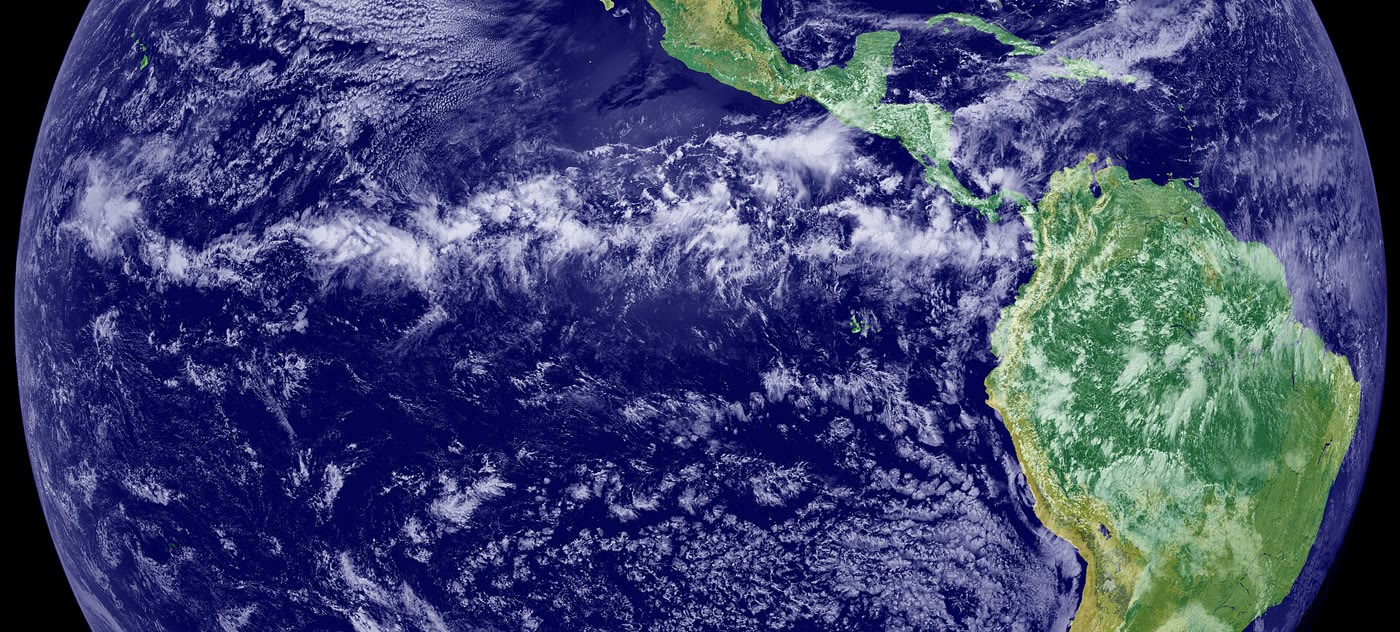
\includegraphics[width=0.8\linewidth]{images/book3/b1-itcz-goes.jpg}

{\small पूर्वी प्रशांत के ऊपर \omterm{def:b1:atmospheric-circulation:itcz}{अंतरोष्ण अभिसरण क्षेत्र}: भूमध्य रेखा के उत्तर में महासागर पार करती चमकीले मेघों की एक रेखा, मध्य और दक्षिण अमेरिका दाईं ओर। चित्र GOES-11 भू-स्थिर उपग्रह के मेघ-आँकड़ों को भू-आवरण के रंगों के साथ मिलाता है। (फ़ोटो: NASA Earth Observatory, सार्वजनिक डोमेन, विकिमीडिया कॉमन्स के माध्यम से।)}
\label{fig:b1:atmospheric-circulation:itcz-photo}
\end{omfigure}
% ledger: commons:itcz-goes

अभिसरित होती वायु को उठना होता है, और उठती नम वायु मेघ बनाती है: ITCZ ग्रह की सबसे वर्षा-समृद्ध पट्टी है, और उसकी स्थिति उस \omterm{def:b1:spherical-astronomy:geographic}{अक्षांश} से पता चलती है जहाँ ज़ोनल माध्य वर्षा शिखर पर है। ITCZ सूर्य का अनुसरण करता है, कुछ विलंब से। पुनर्विश्लेषण में शिखर फ़रवरी में \ang{12.8} दक्षिण से सितंबर में \ang{10.9} उ तक चलता है; बारह महीनों पर औसत लेने पर वह \ang{2.6} उ पर है। ज़ोनल माध्य देशांतरों के बीच बड़े अंतर छिपा देता है: छायाचित्र में पूर्वी प्रशांत पर पट्टी भूमध्य रेखा के उत्तर में है, और ज़ोनल माध्य ऐसी पट्टियों को उन अन्य के साथ औसत करता है जो ऋतुओं के साथ और दूर झूलती हैं।
% ledger: data:b3-ncep (computed in figdata/bachelor-1/general_circulation.py)

\begin{omfigure}
\begin{tikzpicture}
\begin{axis}[omrecord, width=0.7\linewidth, height=5.2cm, xmin=0.5, xmax=12.5, ymin=-16, ymax=16,
  xlabel={महीना}, ylabel={अक्षांश (\unit{\degree})}, xtick={1,...,12},
  xticklabels={J,F,M,A,M,J,J,A,S,O,N,D}, ytick={-15,-10,...,15}]
% figdata/bachelor-1/general_circulation.py; ledger: data:b3-ncep
\addplot[black!40, domain=0.5:12.5] {0};
\addplot[omThm, line width=1.1pt, mark=*, mark size=1.6pt] table[x=month, y=lat] {figdata/out/bachelor-1-general_circulation-itcz.dat};
\end{axis}
\end{tikzpicture}

{\small क्षेत्र-माध्य वर्षा-शिखर का \omterm{def:b1:spherical-astronomy:geographic}{अक्षांश}, महीने-दर-महीने, \ang{20} दक्षिण और \ang{20} उ के बीच: \omterm{def:b1:atmospheric-circulation:itcz}{अंतरोष्ण अभिसरण क्षेत्र} उत्तरी ग्रीष्म में उत्तर की ओर और दक्षिणी ग्रीष्म में दक्षिण की ओर खिसकता है, सूर्य से दो या तीन महीने पीछे। एनसीईपी-एनसीएआर पुनर्विश्लेषण 1, 1991--2020 के माध्य, डेटा: NOAA PSL।}
\label{fig:b1:atmospheric-circulation:itcz}
\end{omfigure}
% ledger: data:b3-ncep

भूमध्य रेखा पर स्वयं, जहाँ $f = 0$ है, वायु सीधे दाब-प्रवणता के नीचे चलती है, और प्रशांत पर एक पूर्व--पश्चिम परिसंचरण प्रकट होता है।

\begin{definition}[वॉकर परिसंचरण]\label{def:b1:atmospheric-circulation:walker}
\emph{वॉकर परिसंचरण}\index{वॉकर परिसंचरण} भूमध्यरेखीय प्रशांत के साथ वायुमंडल का पूर्व--पश्चिम पलटने वाला कोष्ठ है: वायु पश्चिम के गरम पानी के ऊपर, समुद्री महाद्वीप के चारों ओर, उठती है, ऊपर पूर्व की ओर बहती है, पूर्वी प्रशांत के ऊपर नीचे उतरती है और सतह के निकट व्यापारिक पवनों के साथ पश्चिम की ओर लौटती है।
\end{definition}
% ledger: climategov:walker

\begin{omfigure}
\begin{tikzpicture}[>={Stealth[length=2mm]}, font=\scriptsize]
  \fill[blue!12] (0,0) rectangle (11,0.45);
  \shade[left color=orange!45, right color=blue!12] (0,0) rectangle (6,0.45);
  \fill[brown!45] (-0.9,0) rectangle (0,0.6);
  \fill[brown!45] (11,0) rectangle (11.9,0.6);
  \node[anchor=north] at (-0.45,-0.05) {समुद्री};
  \node[anchor=north] at (-0.45,-0.35) {महाद्वीप};
  \node[anchor=north] at (11.45,-0.05) {दक्षिण};
  \node[anchor=north] at (11.45,-0.35) {अमेरिका};
  \node[anchor=north] at (5.5,-0.05) {भूमध्यरेखीय प्रशांत महासागर};
  \node at (1.6,0.22) {गरम पानी};
  \foreach \x in {0.6,1.2,1.8} \fill[black!20] (\x,2.6) circle (0.45);
  \foreach \x in {0.9,1.5} \fill[black!25] (\x,3.0) circle (0.4);
  \draw[line width=1.2pt, omThm, ->] (9.5,0.8) -- (2.0,0.8);
  \draw[line width=1.2pt, omThm, ->] (1.2,1.0) -- (1.2,3.0);
  \draw[line width=1.2pt, omThm, ->] (2.0,3.3) -- (9.5,3.3);
  \draw[line width=1.2pt, omThm, ->] (10.3,3.0) -- (10.3,1.0);
  \node[anchor=south] at (5.75,0.85) {व्यापारिक पवनें, पूर्व से पश्चिम};
  \node[anchor=south] at (5.75,3.35) {ऊपर वापसी प्रवाह, पश्चिम से पूर्व};
  \node[anchor=west, align=left] at (1.6,1.8) {ऊपर उठती वायु,\\भारी वर्षा};
  \node[anchor=east, align=right] at (10.0,1.8) {नीचे उतरती वायु,\\शुष्क};
\end{tikzpicture}

{\small भूमध्यरेखीय प्रशांत के साथ \omterm{def:b1:atmospheric-circulation:walker}{वॉकर परिसंचरण} (योजनाबद्ध; ऊँचाई पैमाने पर नहीं): गरम पश्चिम के ऊपर उठती, ऊपर पूर्व की ओर, पूर्व में नीचे उतरती और सतह के निकट व्यापारिक पवनों के साथ पश्चिम की ओर लौटती।}
\label{fig:b1:atmospheric-circulation:walker}
\end{omfigure}
% ledger: climategov:walker

\omterm{def:b1:atmospheric-circulation:walker}{वॉकर परिसंचरण} स्थिर नहीं है। जब वह दुर्बल होता है, समुद्री महाद्वीप के ऊपर की ऊपर उठती गति दुर्बल होती है और वहाँ की वायु नीचे भी उतर सकती है; जब वह प्रबल होता है, पश्चिम के ऊपर उठना और वर्षा बढ़ती है। ये झूले, एल~नीनो और ला~नीना, और मानसूनों के ऋतु-संबंधी उलटाव, पुस्तक 4 (स्नातक वर्ष 2) का विषय हैं। 1980 के बाद के दशकों में, 2021 का IPCC आकलन \omterm{def:b1:atmospheric-circulation:walker}{वॉकर परिसंचरण} का \emph{अति संभावित} सुदृढ़ीकरण पाता है, जो ला~नीना अवस्था से मिलता-जुलता है, और एक पश्चिम की ओर खिसकाव, परिवर्तनों के आकार में \emph{मध्यम विश्वास} के साथ।
% ledger: climategov:walker, ipcc:hadley-widening

\section{जेट धाराएँ}\label{sec:b1:atmospheric-circulation:jets}

\begin{definition}[जेट धारा; उपोष्णकटिबंधीय और ध्रुवीय-अग्र जेट]\label{def:b1:atmospheric-circulation:jet}
\emph{जेट धारा}\index{जेट धारा} तेज़ पवन की एक संकरी पट्टी है, सामान्यतः क्षोभमंडल में ऊँची एक क्षैतिज पवन, जिसकी स्थिति दिन-प्रतिदिन बदलती है। \emph{उपोष्णकटिबंधीय जेट}\index{उपोष्णकटिबंधीय जेट} \omterm{def:b1:atmospheric-circulation:cells}{हैडली कोष्ठ} की ध्रुवीय किनारी के निकट, सामान्यतः \ang{20} और \ang{30} \omterm{def:b1:spherical-astronomy:geographic}{अक्षांश} के बीच, \qtyrange{12}{14}{km} की ऊँचाई पर पश्चिम से बहता है। \emph{ध्रुवीय-अग्र जेट}\index{ध्रुवीय-अग्र जेट} ध्रुवीय और उपोष्णकटिबंधीय वायु के बीच की सीमा के ऊपर पश्चिम से बहता है, लगभग \ang{50} और \ang{60} के बीच; वह पछुआ पवनों का तीव्र केंद्र है, मध्य-अक्षांशों के अवदाबों और प्रतिचक्रवातों द्वारा निर्देशित और उन्हें निर्देशित करता हुआ।
\end{definition}
% ledger: nws:jets, noaajs:jet

जेट धाराएँ आम तौर पर \qty{9}{km} के आसपास मिलती हैं, \qty{440}{km/h} से अधिक तक पहुँच सकती हैं, और हर गोलार्ध की शीत ऋतु में सबसे प्रबल होती हैं, जब उष्णकटिबंधों और ध्रुव के बीच तापमान का अंतर सबसे बड़ा होता है। \omterm{def:b1:atmospheric-circulation:jet}{उपोष्णकटिबंधीय जेट} \cref{prop:b1:atmospheric-circulation:angular-momentum} का कोणीय-संवेग पवन है, जिसे भँवरों ने नियंत्रित किया है; वह \omterm{def:b1:atmospheric-circulation:cells}{हैडली कोष्ठ} की किनारी पर बैठता है, शीत-माध्य में लगभग \ang{30} के निकट। \omterm{def:b1:atmospheric-circulation:jet}{ध्रुवीय-अग्र जेट} गुज़रते अवदाबों के साथ उत्तर-दक्षिण डोलता है, और गोलार्ध-भर में औसत लेने से वह धुँधला पड़ जाता है: उत्तरी ग्रीष्म के ज़ोनल माध्य में केवल एक दुर्बल शिखर \qty{21.6}{m/s} \ang{42.5} उ के निकट बचता है, और दक्षिणी ग्रीष्म में \qty{29.9}{m/s} \ang{47.5} दक्षिण के निकट। वह पवन जो तब बढ़ती है जब तापमान ध्रुव की ओर गिरता है, ऊँचाई के साथ, तापीय पवन, पुस्तक 5 (स्नातक वर्ष 3) में दिखाई गई है।
% ledger: noaajs:jet, nws:jets, data:b3-ncep-circ (computed in figdata/bachelor-1/general_circulation.py)

\section{अभ्यास}

\begin{exercise}[$\star$]\label{exo:b1:atmospheric-circulation:1}
माना $\Omega = \qty{7.292e-5}{rad.s^{-1}}$। (क)~\omterm{def:b1:atmospheric-circulation:coriolis-parameter}{कोरिऑलिस प्राचल} परिकलित करें
\ang{0}, \ang{30}, \ang{45} और \ang{90} उ पर। (ख)~\ang{45} उ पर \qty{10}{m/s} की पवन का क्षैतिज कोरिऑलिस त्वरण परिकलित करें और उसकी तुलना $g =
\qty{9.81}{m.s^{-2}}$ से करें। (ग)~यदि पवन उत्तर की ओर बहती हो तो वह किस दिशा में इंगित करता है?
% ledger: earth:Trot
\end{exercise}

\begin{exercise}[$\star$]\label{exo:b1:atmospheric-circulation:2}
समुद्र-तल पर दो समदाब-रेखाएँ \qty{4}{hPa} दूर और \qty{400}{km} दूर हैं, जहाँ $\rho =
\qty{1.225}{kg.m^{-3}}$। (क)~\omterm{def:b1:atmospheric-circulation:pgf}{दाब-प्रवणता बल} से उत्पन्न त्वरण परिकलित करें। (ख)~यदि और कुछ कार्य न करता, तो विराम की वायु को \qty{10}{m/s} तक त्वरित करने में कितना समय लगेगा? (ग)~इस त्वरण की तुलना \qty{10}{m/s} की पवन के \ang{45} उ पर कोरिऑलिस त्वरण से करें, और बताएँ कि यह क्या सुझाता है।
% ledger: ussa76:sea-level, earth:Trot
\end{exercise}

\begin{exercise}[$\star$]\label{exo:b1:atmospheric-circulation:3}
\ang{40} उ पर समदाब-रेखाएँ \qty{4}{hPa} दूर और \qty{250}{km} दूर हैं; माना $\rho =
\qty{1.225}{kg.m^{-3}}$। (क)~\omterm{def:b1:atmospheric-circulation:geostrophic}{भू-विक्षेपी पवन} \unit{m/s} में और नॉट में परिकलित करें
(\qty{1}{kn} = \qty{0.5144}{m/s})। (ख)~निम्न दक्षिण में है। पवन किस दिशा से बहती है? (ग)~एक पूर्वानुमानकर्ता जो पवन-बार्ब (दंड और पंख) खींचेगा, उसका वर्णन करें।
% ledger: ussa76:sea-level, earth:Trot
\end{exercise}

\begin{exercise}[$\star$]\label{exo:b1:atmospheric-circulation:4}
पुनर्विश्लेषण के वार्षिक माध्य सतह के निकट पूर्वी पवन \qty{-3.5}{m/s} \ang{15} उ पर, \qty{-4.4}{m/s} \ang{15} दक्षिण पर, \qty{+1.9}{m/s} \ang{45} उ पर और \qty{+6.5}{m/s} \ang{45} दक्षिण पर देते हैं, और समुद्र-तल दाब \qty{1011.8}{hPa} \ang{15} उ पर, \qty{1016.8}{hPa} \ang{30} उ पर और \qty{1015.8}{hPa} \ang{45} उ पर। (क)~चारों अक्षांशों में से हर एक पर पवन-पेटी का नाम दें। (ख)~हर पवन का चिह्न कोष्ठ की सतही शाखा से समझाएँ। (ग)~इन दाबों के अनुसार उत्तरी गोलार्ध का \omterm{def:b1:atmospheric-circulation:cells}{उपोष्णकटिबंधीय उच्च} कहाँ है?
% ledger: data:b3-ncep-circ
\end{exercise}

\begin{exercise}[$\star\star$]\label{exo:b1:atmospheric-circulation:5}
\qty{500}{km} पर \qty{2}{hPa} की दाब-प्रवणता, जहाँ $\rho =
\qty{1.225}{kg.m^{-3}}$, \ang{60}, \ang{50}, \ang{30}, \ang{20}, \ang{10} और \ang{5} उ पर मिलती है। (क)~हर \omterm{def:b1:spherical-astronomy:geographic}{अक्षांश} पर \omterm{def:b1:atmospheric-circulation:geostrophic}{भू-विक्षेपी पवन} परिकलित करें।
(ख)~गहरे उष्णकटिबंध की वास्तविक पवनें ऐसी प्रवणताओं पर शायद ही कुछ मीटर प्रति सेकंड से अधिक होती हैं। समझाएँ कि \omterm{def:b1:atmospheric-circulation:geostrophic}{भू-विक्षेपी संतुलन} भूमध्य रेखा के निकट क्यों विफल होता है, उस समय $1/f$ का उपयोग करते हुए जो कोरिऑलिस बल को पवन मोड़ने में लगता है।
% ledger: ussa76:sea-level, earth:Trot
\end{exercise}

\begin{exercise}[$\star\star$]\label{exo:b1:atmospheric-circulation:6}
(क)~\cref{prop:b1:atmospheric-circulation:angular-momentum} से, भूमध्य रेखा पर विराम में छोड़ी गई वायु-वलय की पवन परिकलित करें, \ang{10}, \ang{15}, \ang{20} और \ang{30} पर; $\Omega a_\oplus = \qty{464.6}{m/s}$ लें। (ख)~वही, उस वलय के लिए जो \ang{10}, \ang{15}, \ang{20} और \ang{30} पर विराम से शुरू होती है। (ग)~उष्णकटिबंधों में \omterm{def:b1:atmospheric-circulation:cells}{हैडली कोष्ठ} की उठती शाखा भूमध्य रेखा पर ठीक रखने के बजाय अक्षांशों पर फैली है। यह अनुमानित जेट को कैसे बदलता है?
% ledger: earth:Trot, earth:Rmean
\end{exercise}

\begin{exercise}[$\star\star$]\label{exo:b1:atmospheric-circulation:7}
(क)~उत्तरी गोलार्ध में एक जहाज़ को दक्षिण-पश्चिम से पवन मिलती है। बाइस बैलट के नियम से, निम्न दाब का केंद्र कहाँ है? (ख)~दक्षिणी गोलार्ध में एक जहाज़ को उत्तर-पश्चिम से पवन मिलती है। निम्न कहाँ है? (ग)~सतह के निकट पवन समदाब-रेखाओं को निम्न दाब की ओर पार करती है। क्या यह (क) के आपके उत्तर को निम्न की दिशा को दक्षिणावर्त या वामावर्त मोड़कर बदलता है?
% ledger: skybrary:buys-ballot
\end{exercise}

\begin{exercise}[$\star\star$]\label{exo:b1:atmospheric-circulation:8}
(क)~\ang{30} उ तक भूमध्य रेखा के बीच और \qty{1000}{hPa} और \qty{100}{hPa} दाब-स्तरों के बीच वायु का द्रव्यमान परिकलित करें, $a_\oplus = \qty{6371}{km}$ के साथ
और $g = \qty{9.81}{m.s^{-2}}$। (ख)~वार्षिक माध्य में पुनर्विश्लेषण का उत्तरी \omterm{def:b1:atmospheric-circulation:cells}{हैडली कोष्ठ} \qty{8.7e10}{kg/s} ले जाता है। उस द्रव्यमान को कोष्ठ से एक बार पार कराने में कितना समय लगेगा? (ग)~शीत-ऋतु कोष्ठ, \qty{21.4e10}{kg/s} के साथ, वही प्रश्न।
% ledger: earth:Rmean, data:b3-ncep-circ
\end{exercise}

\begin{exercise}[$\star\star$]\label{exo:b1:atmospheric-circulation:9}
मान लें कि एक \omterm{def:b1:atmospheric-circulation:cells}{उपोष्णकटिबंधीय उच्च} के नीचे वायु \qty{1}{cm/s} पर नीचे उतरती है, और वह असंतृप्त है। (क)~एक दिन में वह कितना नीचे उतरती है? (ख)~यदि और कुछ कार्य न करता, तो \qty{9.8}{K/km} के \omterm{def:b1:fluid-envelopes-structure:lapse-rate}{शुष्क रुद्धोष्म तापह्रास दर} पर वह एक दिन में कितना गरम होती है? (ग)~वायु हर दिन उतना नहीं गरम होती। \cref{ch:b1:radiation-heat-transport} की कौन-सी प्रक्रिया इस ऊष्मन को संतुलित करती है? (घ)~अनेक महान गरम मरुस्थल इन उच्चों के नीचे क्यों मिलते हैं?
% ledger: nws:dalr
\end{exercise}

\begin{exercise}[$\star\star\star$]\label{exo:b1:atmospheric-circulation:10}
\ang{50} उ पर $f = \qty{1.117e-4}{s^{-1}}$ लें और त्रिज्या
$r = \qty{500}{km}$ के वृत्ताकार समदाब-रेखाएँ (\cref{rem:b1:atmospheric-circulation:gradient})। (क)~उस निम्न के चारों ओर जहाँ \omterm{def:b1:atmospheric-circulation:geostrophic}{भू-विक्षेपी पवन} \qty{15}{m/s} हो, समीकरण $V^2/r + fV =
f|\vec v_g|$ को प्रवणता-पवन $V$ के लिए हल करें। (ख)~एक \omterm{def:b1:atmospheric-circulation:cyclone}{प्रतिचक्रवात} के चारों ओर दिखाएँ कि $V^2/r - fV + f
|\vec v_g| = 0$ का हल तभी है यदि $|\vec v_g| \leq fr/4$, और वह सीमा परिकलित करें। (ग)~(ख) \omterm{def:b1:atmospheric-circulation:cyclone}{प्रतिचक्रवात} के केंद्र के निकट समदाब-रेखाओं के अंतराल के बारे में, अवदाब की तुलना में, क्या संकेत देता है?
\end{exercise}

\begin{exercise}[$\star\star\star$]\label{exo:b1:atmospheric-circulation:11}
(क)~दिखाएँ कि छोटे $\varphi$ (रेडियन में) के लिए भूमध्य रेखा पर विराम में छोड़े गए वलय की पवन
$u \approx \Omega a_\oplus\varphi^2$ है। (ख)~सन्निकटन की तुलना \ang{10} पर सटीक सूत्र से करें, $\Omega a_\oplus = \qty{464.6}{m/s}$ के साथ। (ग)~पुनर्विश्लेषण की \qty{200}{hPa} पर वार्षिक-माध्य पवन \ang{35} उ के निकट \qty{27.0}{m/s} पर शिखर पर है। किस \omterm{def:b1:spherical-astronomy:geographic}{अक्षांश} पर वलय यह गति प्राप्त करेगा? (घ)~उत्तर कोणीय-संवेग तर्क पर कितना भरोसा किया जा सकता है, इसके बारे में क्या कहता है?
% ledger: earth:Trot, earth:Rmean, data:b3-ncep-circ
\end{exercise}

\begin{exercise}[$\star\star\star$]\label{exo:b1:atmospheric-circulation:12}
पुनर्विश्लेषण का ज़ोनल-माध्य वर्षा-शिखर जनवरी से दिसंबर तक निम्न अक्षांशों पर है: \ang{-10.5}, \ang{-12.8}, \ang{-5.8}, \ang{-4.6}, \ang{5.5},
\ang{7.3}, \ang{8.6}, \ang{10.4}, \ang{10.9}, \ang{9.1}, \ang{7.4}, \ang{6.2} (ऋणात्मक: दक्षिण)। (क)~वार्षिक माध्य और परिसर परिकलित करें। (ख)~उपसौर \omterm{def:b1:spherical-astronomy:geographic}{अक्षांश} जून और दिसंबर में चरम पर है। ITCZ उससे कितने महीने पीछे है, और जलवायु तंत्र में कौन-सी चीज़ ऊष्मा संचित कर ऐसा विलंब ला सकती है? (ग)~मान लें कि एक महासागर पर ITCZ वर्ष भर भूमध्य रेखा के उत्तर रहता है। समझाएँ कि ज़ोनल माध्य फिर भी भूमध्य रेखा कैसे पार कर सकता है।
% ledger: data:b3-ncep
\end{exercise}

\section{समस्या: एक मध्य-अक्षांश मौसम-मानचित्र पढ़ना}

\begin{problem}[{सप्ताहांत समस्या --- \ang{50} उ के निकट एक स्टेशन पर पवन}]
\label{pb:b1:atmospheric-circulation:1}
% values: calc/ch28.py (invented map; jet from data:b3-ncep-circ)
उत्तरी अटलांटिक का एक मौसम-मानचित्र \ang{50} उ के निकट स्टेशन P के पास, पश्चिम से पूर्व चलती सीधी समदाब-रेखाएँ दिखाता है, हर \qty{4}{hPa} पर, निम्न दाब उत्तर में है। P \qty{1004}{hPa} और \qty{1008}{hPa} समदाब-रेखाओं के बीच है, जो वहाँ \qty{250}{km} दूर हैं; उसका समुद्र-तल दाब \qty{1006}{hPa} है और वायु का तापमान \qty{10}{\degreeCelsius}। मानचित्र काल्पनिक है, पर उसकी संख्याएँ विशिष्ट हैं।
उपयोग करें $\Omega = 2\pi/(\qty{23.9345}{h})$, $a_\oplus = \qty{6371}{km}$ और शुष्क वायु के लिए $R_d =
\qty{287.05}{J.kg^{-1}.K^{-1}}$, \qty{1}{kn} = \qty{0.514444}{m/s}।

\medskip
\noindent\textbf{भाग I --- दाब-प्रवणता और भू-विक्षेपी पवन।}
\begin{enumerate}
  \item आदर्श-गैस नियम से P पर वायु का घनत्व परिकलित करें।
  \item P पर क्षैतिज दाब-प्रवणता परिकलित करें, \unit{Pa.m^{-1}} में।
  \item \omterm{def:b1:atmospheric-circulation:pgf}{दाब-प्रवणता बल} से त्वरण परिकलित करें।
  \item \ang{50} उ पर $\Omega$ और \omterm{def:b1:atmospheric-circulation:coriolis-parameter}{कोरिऑलिस प्राचल} परिकलित करें।
  \item P पर \omterm{def:b1:atmospheric-circulation:geostrophic}{भू-विक्षेपी पवन} की गति परिकलित करें।
  \item इसे नॉट में और \unit{km/h} में व्यक्त करें।
  \item दिखाएँ कि वह समय जो अकेला \omterm{def:b1:atmospheric-circulation:pgf}{दाब-प्रवणता बल} विराम की वायु को भू-विक्षेपी गति तक ले जाने में लगाएगा, $1/f$ है, और उसे परिकलित करें, साथ में वह समय $2\pi/f$ जो कोरिऑलिस बल एक पूरे वृत्त में पवन को मोड़ने में लेता है।
\end{enumerate}

\medskip
\noindent\textbf{भाग II --- दिशा और गोलार्ध।}
\begin{enumerate}[resume]
  \item P पर \omterm{def:b1:atmospheric-circulation:pgf}{दाब-प्रवणता बल} किस दिशा में इंगित करता है? \omterm{def:b1:atmospheric-circulation:geostrophic}{भू-विक्षेपी पवन} किस दिशा में बहती है, और किस दिगंश से आती है?
  \item बाइस बैलट के नियम से अपने उत्तर की जाँच करें।
  \item P पर खींचे गए पवन-बार्ब का वर्णन करें: दंड की दिशा, पंखों की संख्या, और वे किस ओर खड़े हैं।
  \item मान लें वही समदाब-रेखाएँ, निम्न उत्तर में, \ang{50} दक्षिण पर मिलें। किस दिशा से पवन बहेगी?
  \item वही घनत्व और दाब-प्रवणता के साथ, \ang{30} उ और \ang{60} उ पर \omterm{def:b1:atmospheric-circulation:geostrophic}{भू-विक्षेपी पवन} परिकलित करें।
  \item \ang{5} उ पर परिकलित करें। क्या परिणाम विश्वसनीय है? समझाएँ।
\end{enumerate}

\medskip
\noindent\textbf{भाग III --- सतह पर पवन।} P पर एक वायु-वेगमापी \qty{9.0}{m/s} की पवन मापता है जो समदाब-रेखाओं को \ang{25} पर निम्न दाब की ओर पार करती है।
\begin{enumerate}[resume]
  \item प्रेक्षित पवन और \omterm{def:b1:atmospheric-circulation:geostrophic}{भू-विक्षेपी पवन} का अनुपात, और प्रेक्षित पवन के समदाब-रेखाओं के अनुदिश और उनके आर-पार घटक परिकलित करें।
  \item प्रेक्षित पवन किस दिगंश से बहती है?
  \item \cref{prop:b1:atmospheric-circulation:friction} के रैखिक-घर्षण मॉडल में, कौन-सा समय-स्थिरांक $\tau$ प्रेक्षित कोण देता है, और मॉडल तब कौन-सी गति का पूर्वानुमान करता है? प्रेक्षण से तुलना करें।
  \item \qty{500}{km} त्रिज्या के एक अवदाब के चारों ओर, मान लें कि सबसे निचले किलोमीटर की वायु हर जगह भीतर की ओर बहती है, प्रश्न~14 के समदाब-रेखाओं के आर-पार घटक और प्रश्न~1 के घनत्व के साथ। अवदाब में प्रति सेकंड प्रवेश करने वाली वायु का द्रव्यमान परिकलित करें।
  \item यह वायु परत के शीर्ष से बाहर निकलनी होगी। वहाँ माध्य ऊर्ध्वाधर वेग परिकलित करें, \unit{m/s} में और मीटर प्रति दिन में।
  \item \qty{9.8}{K/km} के \omterm{def:b1:fluid-envelopes-structure:lapse-rate}{शुष्क रुद्धोष्म तापह्रास दर} पर, ऊपर उठती वायु एक दिन में कितनी ठंडी होती है? कौन-सा मौसम उसके बाद आता है, और इसके बजाय \omterm{def:b1:atmospheric-circulation:cyclone}{प्रतिचक्रवात} के नीचे क्या होता?
\end{enumerate}

\medskip
\noindent\textbf{भाग IV --- ऊपर का जेट।} उत्तरी शीत में \qty{200}{hPa} पर ज़ोनल-माध्य पवन \ang{30} उ के निकट \qty{42.3}{m/s} पर शिखर पर है (पुनर्विश्लेषण के माध्य 1991--2020)।
\begin{enumerate}[resume]
  \item भूमध्य रेखा पर और \ang{30} उ पर ज़मीन की पूर्वी गति परिकलित करें।
  \item एक वायु-वलय भूमध्य रेखा पर ऊपर विराम में छोड़ा जाता है और अपना कोणीय संवेग रखता है। \ang{20} उ और \ang{30} उ पर उसकी पवन परिकलित करें।
  \item वही प्रश्न \ang{30} उ पर, उस वलय के लिए जो \ang{10} उ पर विराम से शुरू होता है।
  \item प्रश्न~21 का वलय \ang{30} उ पर प्रेक्षित जेट से कितने गुना आगे निकलता है? असली जेट के धीमे होने के दो कारण दें।
  \item \ang{30} उ पर प्रेक्षित जेट के प्रति इकाई द्रव्यमान निरपेक्ष कोणीय संवेग का भूमध्य रेखा पर विराम की वायु के कोणीय संवेग से अनुपात परिकलित करें। रास्ते में कितना भाग खो गया है?
  \item P पर \omterm{def:b1:atmospheric-circulation:geostrophic}{भू-विक्षेपी पवन} की गति मीटर प्रति सेकंड में क्या है, और सतह पर मापी गई पवन उससे कैसे तुलना करती है?
\end{enumerate}
\end{problem}
